\section{Background}
\label{section:background}

In this section, we provide some basic background information on the types of
\p\ architectures that have been implemented and deployed. We also
describe and motivate more formally the topology mismatch problem 
whose various aspects have been tackled over the past several years.

%%%%%%%%%%%%%%%%%%%%%%%%%%%%%%%%%%%%%%%%%%%%%%%%%%%%%%%%%%%%%%%%%%%%%%%%%%%%%%%%
%%%%%%%%%%%%%%%%%%%%%%%%%%%%%%%%%%%%%%%%%%%%%%%%%%%%%%%%%%%%%%%%%%%%%%%%%%%%%%%%
\subsection{Peer-to-Peer (\p) Overlay Architectures}
%%%%%%%%%%%%%%%%%%%%%%%%%%%%%%%%%%%%%%%%%%%%%%%%%%%%%%%%%%%%%%%%%%%%%%%%%%%%%%%%
%%%%%%%%%%%%%%%%%%%%%%%%%%%%%%%%%%%%%%%%%%%%%%%%%%%%%%%%%%%%%%%%%%%%%%%%%%%%%%%%
Circa 2000, the first file-sharing \p-system introduced the \emph{servent}
concept~\cite{gnutella}, a \emph{portmanteau} that blends the notions of server
and client to denote the dual role of a node participating in the \p-network. 
Such server-less systems have proven to be able to achieve outstanding
aggregate resource capacities as more and more participants join the system
without requiring additional expenditure for infrastructure. 
While certain undesirable features such as 
free-riding~\cite{saroiu_measurefileshare_2002,adar_gnutellafreeriders_2000,hughes_gnutellafreeride_2005},
the distribution of illegal content and other~\emph{socio-technical}
issues \cite{hughes_socp2p_2008}, have arisen, \p\ systems have
continued to gain popularity throughout the years primarily 
because they have successfully supported popular applications 
(i.e. file-sharing) amongst \emph{vast} numbers of participating users.
%%
For over a decade, excitement over the immense potential of \p\ systems has
generated a flurry of research and development, resulting in a wide range of
popular protocols, networks, and applications. As \p\ systems evolved, three
main architectures have emerged, namely
\begin{inparaenum}[\itshape i\upshape)]
  \item \emph{centralized},
  \item \emph{decentralized unstructured}, and
  \item \emph{decentralized structured}.
\end{inparaenum}

Designers of \emph{centralized} architectures 
(Figure~\ref{figure:p2p-archs:centralized}) were the first 
to observe that requests for resources
(e.g., CPU cycles or popular content) need not be sent to
a dedicated server. Instead, such requests could be handled by 
many hosts that already possessed the resources in question. 
The downside of this approach was that it required a 
centralized search directory that invevitably becames a single point of failure,
a scalability bottleneck or a target of malicious behavior such as \emph{DoS}
attacks.

{\sl Napster} was the most successful incarnation of the
centralized approach in file-sharing~\cite{napster}.
It maintained a \emph{central index server} based on file-lists 
that were peer-provided.
Users would query the index server that would ultimately 
yield pointers to the actual content.
Thus, by centralizing search while distributing downloads,  {\sl Napster}
achieved a highly functional design that, at its height, attracted $26$ million
users sharing approximately $80$ million songs\cite{jmm_naptopusage_2001}.
%%
The central indexing component played a vital role in the demise of 
{\sl Napter}, as the \emph{Recording
Industry Association of America} successfully argued in court that this software
entity was enabling copyright infringement of the artists' songs exchanged
through the system.

Architectures that distributed both search and resource provision 
capabilities (Figure~\ref{figure:p2p-archs:unstructred-full}) soon followed.
In these \emph{decentralized} approaches, 
resource placement within the overlay topology is random~\cite{YG-M2002};
for this reason, such architectures are referred to as \emph{unstructured}. 
Key properties of such \p\ systems are that they support inherent heterogeneity
of peers, are highly resilient to peer failures, and incur low maintenance
overhead at handling the dynamics of peer participation
\cite{stutzbach_churn_2006}. Unstructured systems are also known as 
\emph{broadcast-based} systems as they use message flooding among
peers to propagate search queries. 
In its first realization,
{\sl Gnutella}(\emph{v.0.4}) is a well-known example of the fully
decentralized unstructured approach.

A key disadvantage of the unstructured approach is that message flooding burdens
the network since queries travel within the network randomly, visiting nodes
that do not have the sought resource and thus wasting bandwidth.  
To save on bandwidth, unstructured networks typically limit how long 
a query travels within the overlay via the \emph{time-to-live} parameter
(\emph{TTL}). 
When a query is received by a node, it decreases its \emph{TTL} by one unit. 
If the \emph{TTL} has not reached zero, the node forwards the query 
to its neighbors.  Otherwise, it drops the query. 
While this approach prevents queries from visiting the entire network, it
does not guarantee that the resource of interest, (e.g., a rare recording)
will, ultimately, be found.
%%%
\begin{figure}[ht]
\centering
\subfigure[Centralized ({\sl SETI@Home} or {\sl Napster}). Peers query the centralized
entity (dotted lines) and then establish the connection to the data source.] {
  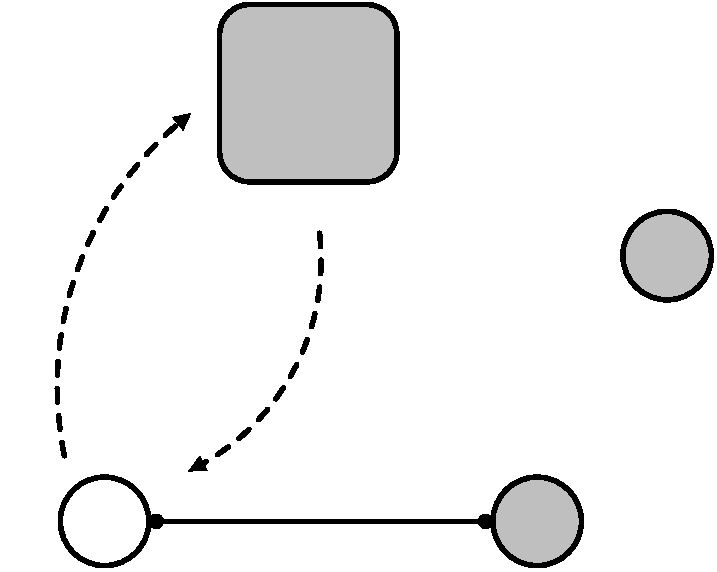
\includegraphics[scale=0.20]{img/pdf/centralized.pdf}
  \label{figure:p2p-archs:centralized}
}\qquad\qquad
\subfigure[Fully unstructured ({\sl Gnutella} \emph{v.0.4}). Data is distributed randomly,
the topology is also random and all participants are equal.] {
  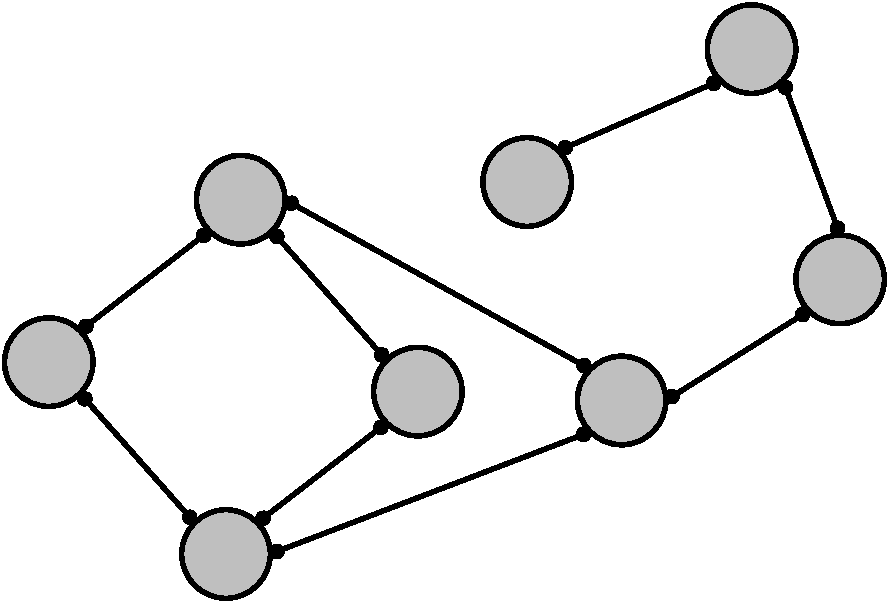
\includegraphics[scale=0.20]{img/pdf/unstructured-full.pdf}
  \label{figure:p2p-archs:unstructred-full}
}\qquad\qquad
\subfigure[Hierarchical unstructured ({\sl Gnutella} \emph{v.0.6} or {\sl FastTrack}). Certain
peers (bigger circles) shoulder specific responsibilities (e.g., data
indexing).] {
  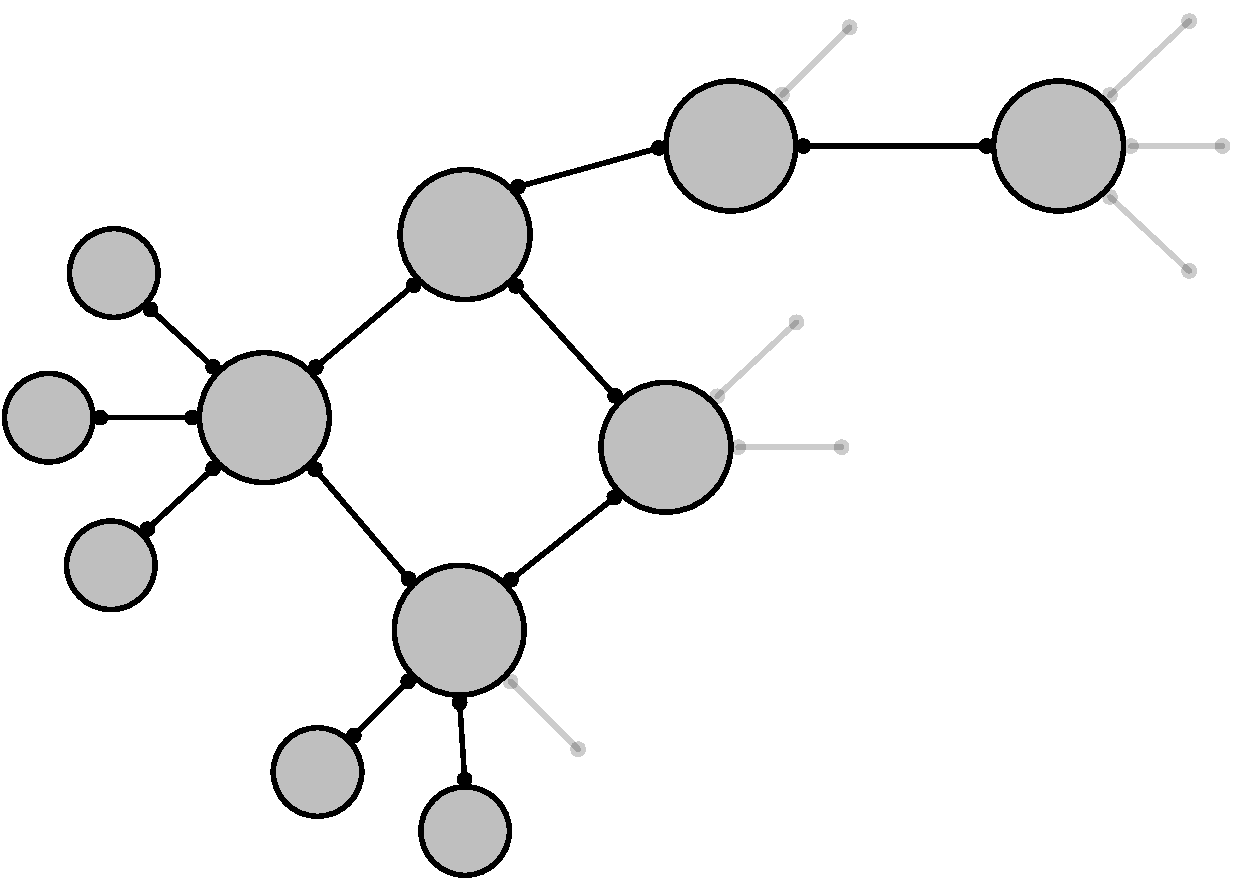
\includegraphics[scale=0.20]{img/pdf/unstructured-hierarchical.pdf}
  \label{figure:p2p-archs:unstructured-hierarchical}
}\qquad\qquad
\subfigure[Structured ({\sl Chord} and {\sl Kademlia}). 
Peers and data are placed in the overlay in a deterministic manner.] {
  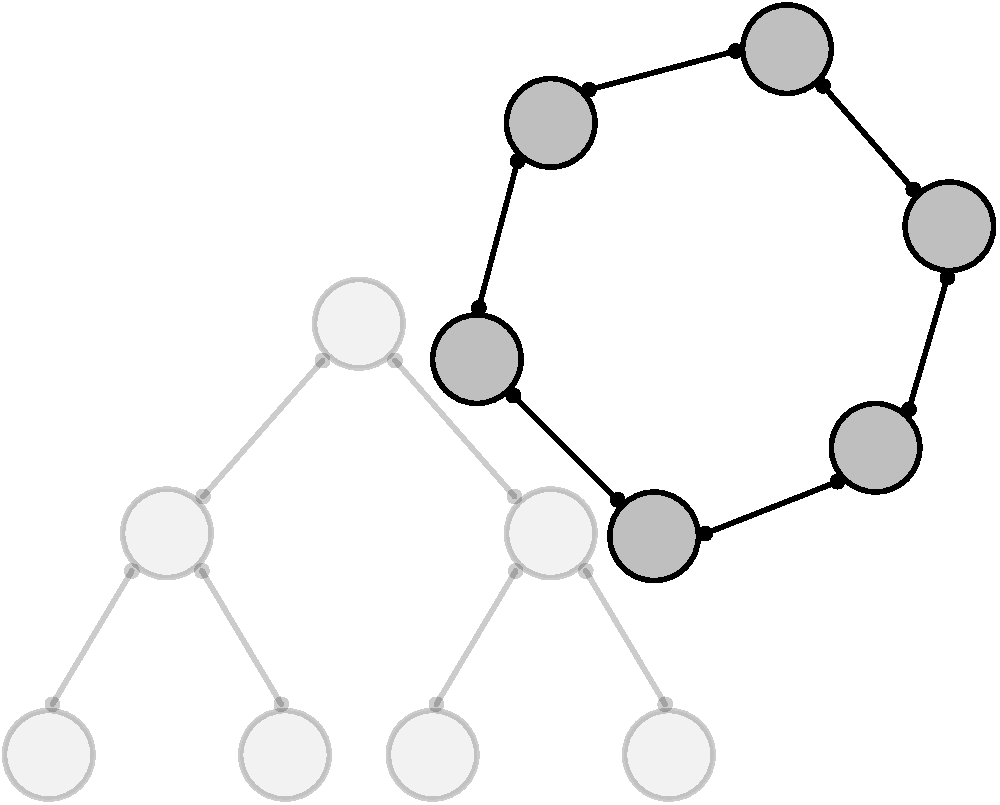
\includegraphics[scale=0.20]{img/pdf/structured.pdf}
  \label{figure:p2p-archs:structured}
}
\caption{The various \p\ architectures.}
\label{figure:p2p-archs}
\end{figure}

%%%%%%%%%%%%%%%%%%%%%%%%%%%%%%%%%%%%%%%%%%%%%%%%%%%%%%%%%%%%%%%%%%%%%%%%%%%%%%%%

To shorten search times, improve scalability, and lighten network load, 
unstructured configurations evolved into \emph{hierarchical} systems 
that dynamically assigned indexing functions to special peers, 
called \emph{ultra-}  or \emph{super-peers} 
(Figure~\ref{figure:p2p-archs:unstructured-hierarchical}). 
Peers with reliable network connections and/or high compute power 
became \emph{ultra/super-peers}
facilitating less-powerful \emph{leaf-nodes} to find resources of
interest. 
Examples of such hierarchical unstructured systems include
{\sl Gnutella}(\emph{v.0.6})/{\sl Limewire}~\cite{gnutella}, 
{\sl KaZaA}~\cite{kazaa} and {\sl Skype}~\cite{skype}. 
Although the hierarchical approach relieves network pressure as
search queries were flooded over the much smaller subset of 
ultra/super-peers, it fails to address the reduced search scope and
inability to locate rare resources.

\emph{Decentralized structured schemes} were introduced as an answer to the above
problems of decentralized unstructured \p--approaches
(Figure~\ref{figure:p2p-archs:structured}).
Here, the main objective was to offer 
a self-organizing infrastructure for large-scale \p\ applications
\cite{ratnasamy_can_2001,stoica_chord_2001,antony_pastry_2001,zhao_tapestry_2001,maymounkov_kademlia_2002,rgrk_bamboo_2004}.
To achieve that, they implement a \emph{Distributed Hash Table (DHT)} that maps
objects to nodes through a deterministic mechanism. \emph{DHT}s provide a
guaranteed bound on the number of overlay routing hops that have to be
``traveled'' to locate a resource, even in the case when only a \emph{single}
copy exists whithin the system. This requires
$O$($log(n)$) hops, compared to the unstructured networks that require
$O(n)$ to reliably locate any object. Unfortunately this efficiency does not
come without cost. Structured overlays can only support exact-match queries 
(i.e., queries that identify resources by name) as opposed
to content-based retrieval provided by unstructured overlays. 
This means that unstructured overlays can support more versatile 
resource location queries such as keyword and partial matching searches. 
Several popular file-sharing \p\ applications have been based on \emph{DHT}s
including {\sl Overnet}/{\sl eDonkey}~\cite{overnet}, 
{\sl Kademlia}/{\sl Kad Network}~\cite{maymounkov_kademlia_2002},  and 
some flavors of {\sl BitTorrent}~\cite{c_bittorrent_2003}.  
Moreover, \emph{DHT}s sparked
a flurry of research for many, diverse, applications ranging
from distributed search engines to event-notification and cloud-based
platforms~\cite{kbc_oceanstore_2000,rkcd_scribe_2001,mgpj_cloudsnap_2011}.

%
% TODO: SOME DISCUSSION ON P2P ARCHITECTURES
%
%\cite{matei_mapgnutella_2002, LCCLS2002, merugu_str2unstr_2003}
%showed that the ad-hoc network topology of unstructured overlay networks that
%preserve \emph{Power Law} and \emph{Small World} characteristics\footnote{Power
%Law describes the node degree while the Small World describes characteristics
%of path length and clustering coefficient. The clustering coefficient for a
%node $\upsilon$ in a graph $G = \left( V, E \right)$ is defined as the ratio of
%the existing connections between $\upsilon$'s neighboring nodes to $\gamma
%\times \left( \gamma - 1 \right)$, where $\gamma$ is the number of neighboring
%nodes of $\upsilon$. High cluster coefficient means that neighboring nodes of
%any node $\upsilon$ likely connect one another.} \cite{faloutsos_powerlaw_1999,
%saroiu_measurefileshare_2002} offer a more promising approach. Particularly:
%\begin{itemize}
%  \item Peer-to-peer clients are extremely \emph{transient}. Unstructured
%systems can have high maintenance traffic in delivering messages, updating the
%mapping, discovering failures and replicating lost data or pointers, making
%them insufficient on highly volatile networks.
%  \item \emph{Keyword searches} versus \emph{exact-match queries}. In DHTs
%there is a tight control between the data placement and the topology of the
%network. For this reason it is hard to efficiently support partially matched
%queries while Gnutella and other similar systems effortlessly support keyword
%searches and other complex queries since the mechanism is realized locally, on
%a node-by-node basis.
%  \item Popular content is located at multiple peers and thus it is more likely
%for a flooding-based search to return results. DHTs, on the other hand, fit
%better in the systems which require ability to reliably locate content, even in
%the extreme case that only a single-copy exists in the network.
%\end{itemize}

%
% TODO: SOME DISCUSSION ON THE ADVANTAGES OF UNSTRUCTURED NETWORKS FROM
%       \cite{z-yk_ddno_2005}
%
%Unstructured P2P networks o?er a number of
%important advantages: (i) An unstructured network
%imposes very small demands on individual nodes,
%and more specifically?cally it allows nodes to join or leave
%the network without signi?cantly a?ecting the sys-
%tem performance. (ii) Unstructured networks are
%appropriate for content-based retrieval (e.g., key-
%word searches) as opposed to object identi?er loca-
%tion of structured overlays. (iii) Finally unstructured
%networks can easily accommodate nodes of vary-
%ing power. Consequently, they scale to very large
%sizes and they o?er more robust performance in
%the presence of node failures and connection
%unreliability.
%

%
% TODO: SOME DISCUSSION ON STRUCTURED OVERLAYS PROBABLY FROM
%       \cite{WLH2007}
% However, the design of a decentralized but structured P2P network has to
% overcome two critical issues. The first issue is the long routing latency.
% Several proximity schemes  have been proposed to avert long routing latency in
% current structured P2P networks, but they require a high-complexity procedure
% to periodically maintain the routing table (e.g. Pastry system) or they need
% pre-chosen landmarks to construct the overlay. However, the P2P system is by
% its very nature unstable since nodes join and leave frequently. For instance,
% the study of Gnutella shows around approximately 1200 membership changes per
% minute in a 100 000 nodes P2P system. Another proximity scheme needs some
% pre-chosen landmarks or a complete BGP routing table support. As a result,
% they both increase the difficulty of the P2P system deployment. The second
% issue is system maintenance overhead. The existing structured P2P networks
% allow nodes to keep some nearby nodes in their routing tables in order to
% achieve efficient routing.
%


%%%%%%%%%%%%%%%%%%%%%%%%%%%%%%%%%%%%%%%%%%%%%%%%%%%%%%%%%%%%%%%%%%%%%%%%%%%%%%%%



%%%%%%%%%%%%%%%%%%%%%%%%%%%%%%%%%%%%%%%%%%%%%%%%%%%%%%%%%%%%%%%%%%%%%%%%%%%%%%%%
%%%%%%%%%%%%%%%%%%%%%%%%%%%%%%%%%%%%%%%%%%%%%%%%%%%%%%%%%%%%%%%%%%%%%%%%%%%%%%%%
\subsection{The Topology Mismatch Problem}
%%%%%%%%%%%%%%%%%%%%%%%%%%%%%%%%%%%%%%%%%%%%%%%%%%%%%%%%%%%%%%%%%%%%%%%%%%%%%%%%
%%%%%%%%%%%%%%%%%%%%%%%%%%%%%%%%%%%%%%%%%%%%%%%%%%%%%%%%%%%%%%%%%%%%%%%%%%%%%%%%

One of the major issues that defines the efficiency of 
an overlay network is its mapping to 
the underlying physical infrastructure. 
Recall, in Figure~\ref{figure:overlay} nodes $A$ and $B$ are 
on the same local network, while $C$ and $D$ are in different networks. 
The top layer represents the overlay interconnection formed by 
these four nodes at a higher level. 
Link connections there, can change as needed by 
the running environment, without any
particular constraint by the underlying physical topology. 
%%
For instance, assume nodes $A$, $B$, $C$ and $D$ being 
connected via the physical network shown in Figure~\ref{figure:phys}
in which costs are depicted in milliseconds. 
%%
\begin{figure}[ht]
\centering
  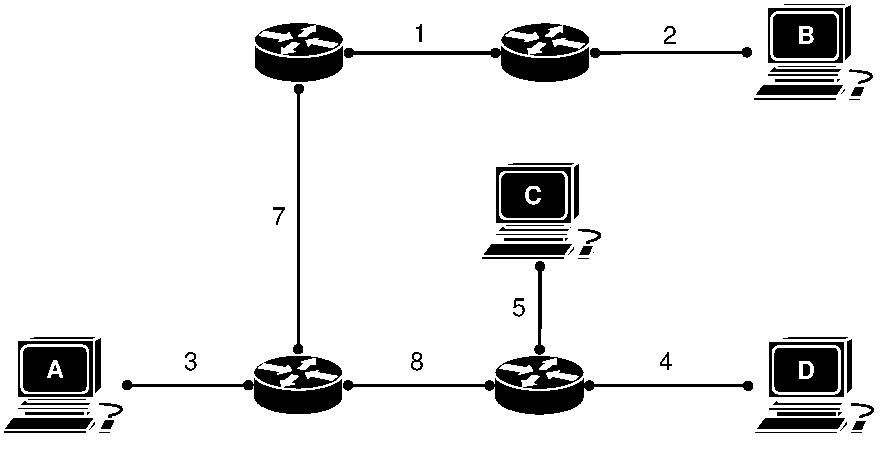
\includegraphics[scale=0.4]{img/pdf/example-physical.pdf}
\caption{Interconnection of nodes in the physical level.}
\label{figure:phys}
\end{figure}
%%
When peer $A$ sends a message its $D$ counterpart
and depending on the overlay configuration, 
nodes will experience different performance.
For example, in the overlay depicted in
Figure~\ref{figure:overlay-1}, the
message will traverse the following sequence of links in the physical layer
(marked with their costs): $3 \rightarrow 7 \rightarrow 1 \rightarrow 2
\rightarrow 2 \rightarrow 1 \rightarrow 7 \rightarrow 8 \rightarrow 5
\rightarrow 5 \rightarrow 4$. In the alternative overlay of
Figure~\ref{figure:overlay-2}, the path will be: $3 \rightarrow 8 \rightarrow
4$. 
The respective costs are $45 ms$ and $15 ms$.
Evidently, the second overlay is more
congruent with the underlying physical network in comparison 
to the first and, thus, is more efficient. 

\begin{figure}[ht]
\centering
\subfigure[Nodes $B$ and $C$ have direct overlay connection.] {
  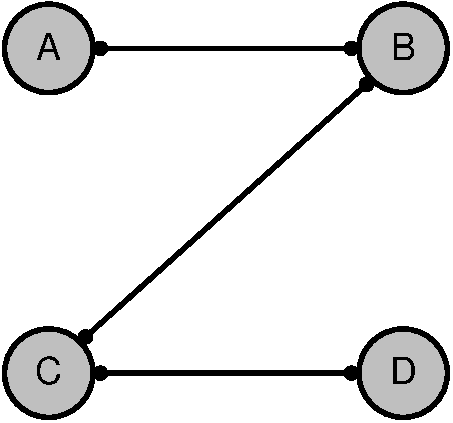
\includegraphics[scale=0.4]{img/pdf/example-overlay-inefficient.pdf}
  \label{figure:overlay-1}
}\qquad\qquad
\subfigure[Nodes $A$ and $D$ have direct overlay connection.] {
  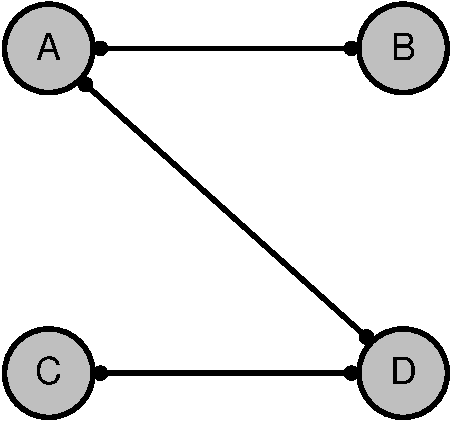
\includegraphics[scale=0.4]{img/pdf/example-overlay-efficient.pdf}
  \label{figure:overlay-2}
}
\caption{Two different overlay connection configuration.}
\label{figure:overlay-confs}
\end{figure}

Ideally, an overlay should be constructed to achieve an \emph{optimal} 
mapping with its underlying network links, to avoid
inefficient states where redundant physical resources are utilized for the
operation of the same virtual link in the overlay. The ratio of the actual
\emph{IP} network distance a message travels to reach an object of interest
(via overlay routing) to the minimal \emph{IP} network distance to that object
(i.e. through \emph{IP}) is known as \emph{stretch} or
\emph{Relative Delay Penalty (RDP)}~\cite{CRZ2000}.

The problem of constructing an optimal overlay is referred to as the
\emph{topology mismatch problem}, and is formally defined as follows:

%%VM: Are we 100\% sure about the definition?
\begin{definition}
Let $V$=$\{v_1$, $\dots$, $v_n\}$ be a set of points denoting the network nodes,
$\{v_i, v_j\} \in E$ be the set of unicast distances between nodes $v_i$ and
$v_j$, $G=(V,E)$ be a complete distance graph over $V$. The topology mismatch
problem is to construct a minimal spanning tree, where node degree is
restricted to a constant ($k\geq 2$) by the bandwidth of each node $v_i$.
\end{definition}

Early overlay protocol implementations did not pay to much attention to map
optimally to the underlying network topology. {\sl Gnutella}, for example, is
considered far from scalable~\cite{ritter_gnucantscale_2001} since every peer
chooses its neighbors without any knowledge of the underlying
network, resulting in mismatch. 
Queries may be flooded over multiple paths merging in one peer 
while one of the paths would suffice.  
Moreover, peers may forward the same message to each other
before they receive the query messages from each other.
\cite{matei_mapgnutella_2002} showed that, even when $95$\% of any two nodes 
are less than $7$ hops away from each other, 
a \emph{flooding-based} {\sl Gnutella}-like algorithm 
can generate $330$TB/month in a $50,000$ node network. 
A topology mismatch can thus have a serious effect 
on Internet's router performance.

Similar problems are observed in decentralized structured schemes as well.
Typically, node IDs are assigned \emph{randomly}, resulting in excellent load
balancing, scalability, and robustness for the overlay. Unfortunately, this
randomness has a negative impact on the \emph{routing locality} of the network.
This means that even though the target node can be reached with a logarithmic
number of overlay hops, the distance traveled in the underlying network, 
during the overlay routing process, can be far from optimal.  

%%%%%%%%%%%%%%%%%%%%%%%%%%%%%%%%%%%%%%%%%%%%%%%%%%%%%%%%%%%%%%%%%%%%%%%%%%%%%%%%
%%%%%%%%%%%%%%%%%%%%%%%%%%%%%%%%%%%%%%%%%%%%%%%%%%%%%%%%%%%%%%%%%%%%%%%%%%%%%%%%
\subsection{Motivation and Goal for this Survey}
%%%%%%%%%%%%%%%%%%%%%%%%%%%%%%%%%%%%%%%%%%%%%%%%%%%%%%%%%%%%%%%%%%%%%%%%%%%%%%%%
%%%%%%%%%%%%%%%%%%%%%%%%%%%%%%%%%%%%%%%%%%%%%%%%%%%%%%%%%%%%%%%%%%%%%%%%%%%%%%%%
A topology--unaware overlay network is able to control the sequence of peers a
message traverses before reaching its destination, but it completely ignores
how the actual packets are switched at the underlying infrastructure along
the overlay path. 
In particular, a single logical point-to-point link on the
overlay typically corresponds to multiple physical links in the
underlying layer. 
Moreover, a link in the physical network often lies
on several overlay paths inadvertently increasing the traffic on that
link; this is known as the link's \emph{stress}~\cite{CRSZ2002}. 
There is also the stochastic phenomenon during which peers 
depart and others arrive in the network, known 
as \emph{churn}~\cite{stutzbach_churn_2006}.
Even when an approach offers the best possible location
when a node joins in, the churn is set to  
continuously undermine the effort to maintain the best possible position
of the  peer in the network.

The topology mismatch problem is exacerbated by the extremely large amounts of
traffic generated by highly popular \p\ applications~\cite{byl-book}.
Addressing this problem remains a fundamental challenge 
in contributing to the overall efficiency of the Internet. 
Unfortunately, topology mismatch is known to be 
an \emph{NP-Hard} problem \cite{C2000,NPBOOK}. 
There is also additional complexity due to the fact that 
end-to-end latencies demonstrate \emph{triangle inequality
violations (TIVs)} which are a consequence of the Internet's structure and
routing policies; as such, they will remain a property of the Internet 
for the foreseeable future \cite{zheng_irprtt_2005}. 
\emph{TIV}s affect both network coordinate
\cite{cox_vivaldi_2004,WSS2005} and positioning \cite{ng_gnp_2001}
systems and makes the construction of \emph{IP}-topology-aware 
overlays difficult.

Over the past several years, researchers have investigated an extensive
array of heuristic solutions to the topology mismatch problem. 
The purpose of this survey is to gather and organize 
this extensive body of produced knowledge. 
We aspire to assist the reader in better understanding the 
different approaches suggested and to accomplish this we 
present methods for both structured and unstructured distributed 
overlay networks.
We outline the respective algorithmic aspects and we categorize
the surveyed material so that pros and cons of each method
can become apparent in their context.

We employ both tabular and pictorial means to 
articulate features of the proposed methodologies and outline
both strengths and weaknesses.
To ascertain the effectiveness of each proposal, we predominantly use 
three criteria that capture the behavior of the algorithms 
discussed:
\emph{efficiency}, \emph{overhead} and \emph{scalability}.
For each of these criteria, we use a coarse-grained,
three-level, gradation to denote how well the algorithms do,
namely \emph{low}, \emph{medium} and \emph{high}.
Each criterion has its own
interpretation of the above literal values. 
\emph{Efficiency} means how well the
algorithm performs its search and topology adaptation functions. We also take
take into account how this might effect other characteristics of the networks
under consideration\footnote{For example we don't actually want a topologically
optimized BitTorrent swarm if this results in a degraded download performance,
a characteristic that is the protocol's corner stone.}.
%%VM Does the above sentence with the footnote now connect?
%%
%% PREVIOUS COMMENT AD I am not sure what the above line says.. or connects. Something is
%%	missing...

%% SOME ADDITIONAL EXAMPLES FOR EFFICIENCY IF WE WANT TO ADD THEM
%minimum-spanning-tree-based techniques have slow convergence speed in topology
%adaptation or the high clustering impacts load balancing and constrains search
%scope (or at least increases search satisfaction time), all reducing overall
%efficiency. 

Moreover, efficiency is negatively effected every time an algorithm
reduces its search scope.
For the \emph{overhead} criterion, we evaluate the cost
to compute and communicate peer join, message forwarding, 
and topology maintenance. For example, when a protocol relies on peers
exchanging routing tables with other peers within a 2-hop radius with each other
, then we can be safelly deduce that it incurs lower overhead when compared to a
protocol that requires global knowledge of the overlay network.
%%VM Does the above sentence with the footnote now connect?
%%
%%PREVIOUS COMMENT AD Again I am not sure how the example above ties with the definition...
For the \emph{scalability} criterion, we consider system behavior 
with respect to the number of participating peers. 
We consider systems with low, medium, and high scalability 
to mean they can support hundreds, tenths of thousands, 
and millions of nodes, respectively. 
